In this chapter I explain each step taken during the pre-processing phase, by illustrating in details each step taken and tool used. \newline
\par
My work is focused on the first phase of a data analysis procedure which is the pre-processing.
Data pre-processing (or data preparation) is the process of transforming raw data into a suitable format for modelling. 
Indeed, raw data is in most cases incomplete and noisy.\par
Nowadays, dealing with big amount of information, the probability of incorrect data is higher without a proper data pre-processing.
Only high-quality data can generate accurate models and predictions. \par
The view and quality of data is very relevant before running any analysis.
Hence, it’s crucial to process data with the best possible quality before training them with artificial intelligence, and machine learning predictive models.\par
\section{Data Collection}
Data collection is the process of gathering information in variables of interest for answering relevant questions. \newline
Relevant data is gathered from their sources and merged in data structures (such as Dataframes). In our work, data come from fixed ground-sensor, satellite-based platform, models and map layers. In this phase are processed (mostly) numerical and categorical data. 
\section{Data Cleaning}
\label{sec:Data cleaning}
Data has to be prepared in accordance with the supervised feature selection.
Data cleaning aims to fix problems or errors in messy data. There are many reasons data may have incorrect values, such as being corrupted, duplicated or invalid. \newline
This could be done by removing rows or columns. Alternately, it might involve replacing observations with new values. \newline

\subsection{Remove of variables with low variance}
An approach for removing columns is to consider the variance of each column variable. The variance is a statistic representing the expected value of the squared deviation from the mean $\mu$ of a given variable X. 
\begin{equation}
  Var(X) = E[(X-\mu)^2]
\end{equation}
The variance can be used as a filter for identifying columns to be removed from a given data set. 
Using a feature with low-variance only adds complexity and noisy to the feature selection and the predictive.\newline
In order to do that, I performed VarianceThreshold method from the scikit-learn library. In this way, features under a certain variance threshold value should be meaningless and consequently discarded by its dataset. 
\section{Data Transformation}
Data need to be scaled. As a matter of fact, each feature in our data has varying degrees of magnitude, range, and units. This is an issue for machine learning algorithms because of highly sensitive to these features. 
Having input variables with different units (e.g. ug/m\textsuperscript{3}, °C, hours or mol/m\textsuperscript{2}) implies data at different scales. This could raise the difficulty of the problem being modelled. \newline
Hence, a common scale through Normalization or Standardization is needed in order to improve the data quality.\newline
Many ML and regression algorithms perform better when numerical input and output variables are scaled to a common standard range. \newline
For instance, it's proved that neural networks trained with scaled data performs better in terms of MSE \cite{shanker1996effect}.
In this step, two type of transformation have been done:
\subsection{Standardization}
The most common data transformation is to centre and scale the each variable values. In order to do that, the average value is removed from all the values. As a result of centring, the predictor will have a zero mean.\cite{kuhn2013applied}
Standardization consists in rescaling data following a Gaussian distribution of values with mean equals to 0 and standard deviation equals to 1:
\begin{equation}
  Z = \frac{X-\mu}{\sigma}
\end{equation}
\begin{equation}
\mu = \frac{(\sum_{n=1}^{N} X_i)}{N}
\end{equation}
\begin{equation}
\sigma = \sqrt{\frac{(\sum_{n=1}^{N} X_i-\mu)}{N-1}}
\end{equation}
Where:
\begin{itemize}
\item Z is the numeric value standardized of a given covariate;
\item X is the numeric value to be standardized of a given covariate;
\item $\mu$ is the mean value for the set of values assumed by a given covariate;
\item $\sigma$ is the standard deviation for the set of values assumed by a given covariate;
\end{itemize}
Every terms was computed by using Scipy library (scipy.stats). 
\bigbreak
\subsection{Normalization}
Data Normalization is a different methods process for adjusting data at different scales. Data a scaled in a range between 0 and 1 and was performed only for the feature selection methods output.
Output normalization is an essential step for the comparison of different output, since data ranges vary for each method used.\newline
This was performed in my Notebooks from the scikit-learn library (sklearn.preprocessing) through the MinMaxScaler method.
\section{Feature Selection}
Feature Selection is the core part of this study. It's the process of reducing the number of input variables when developing a predictive model by basing on a target (or output) variable. 
Data collected, even if have been cleaned and transformed, are anyway characterized by big amount of variables which are redundant.
Discarding irrelevant data is essential before applying Machine Learning model in order to:
\begin{itemize}
\item \textbf{Reduce Overfitting}: less opportunity to make decisions based on noise;
\item \textbf{Improve Accuracy}: less misleading data means that modelling accuracy improves. Predictions can be greatly distorted by redundant attributes;
\item \textbf{Reduce Training Time}: With less data an algorithm will train faster;
\end{itemize}
In this step, which will be explained in detail in the next chapters, the reduced input variables are the ones that are meaningless with respect to a target variable as output. \newline
Due to the fact that there isn’t a best feature selection technique, many different methods are performed, each one that gives different correlation results.\par
In the following subsection each FS method implemented is described in detail, classified in three main categories\cite{stanczyk2015feature}, as we can find in literature:
\subsection{Filter Methods}
Filter-based feature selection methods adopt statistical measures to evaluate the correlation/dependence between input variables.\newline
These select features from the without machine learning algorithm. In terms of computation, they are very fast and are very suitable in order to remove duplicated, correlated, redundant variables\cite{saeys2007review}. \newline
These methods evaluate each feature individually without considering the interaction between them. Therefore, they don't fit well if data has high multicollinearity\cite{daoud2017multicollinearity}.

\subsubsection{Pearson coefficient}
Pearson coefficient is one of the most widely used indices for measuring linear correlation in statistics. It ranges between -1 and 1, where:
\begin{itemize}
\item 1 indicates a strictly positive correlation;
\item -1 indicates a strictly negative correlation;
\item0 indicates no correlation between the features;
\end{itemize}

Therefore, by taking only its absolute value, 1 implies that a linear equation describes the relationship between X and Y perfectly, for both positive and negative correlation. \newline
The Pearson index between and independent variable X and a target variable Y is defined by the following formula:

\begin{equation}
  \rho_{x,y} = \frac{Cov(X,Y)}{\sigma_x\sigma_y}
\end{equation}

\subsubsection{Kendall Tau}
Kendall Tau index is used to measure monotonic relationship as test statistic to determine whether two variables are statistically dependent. \newline
While in the linear correlation two variables move together at a constant rate, monotonic or rank correlation measure how likely two variables move in the same direction, but not necessarily in a constant manner. \newline
Like Pearson’s correlation, Kendall’s has a value between -1 and 1, where:

\begin{itemize}
\item -1 represent a strictly negative monotonic relationship;
\item 1 represent a strictly positive monotonic relationship;
\item 0 representing no relationship;
\end{itemize}
Given a sample X and Y with n as sample size, tau index is computed through the formula:
\begin{equation}
  \tau_{x,y} = \frac{n_c-n_d}{\frac{1}{2}n(n-1)}
\end{equation}
where:
\begin{itemize}
\item n\textsubscript{c} = \# of concordant value (concordant value: value are ordered in the same way);
\item n\textsubscript{d} = \# of discordant value (discordant value: value are ordered differently);
\end{itemize}
\subsubsection{Spearman Rho}
Spearman’s index is very similar to Kendall’s. As the previous filter methods, it ranges between -1 and 1, and it's considered less robust than Kendall's.
It's computed in this way:
\begin{equation}
\rho_{x,y} = \frac{6\sum_{n=1}^{N} d_i^2}{n(n-1)^2}
\end{equation}
\begin{itemize}
\item d\textsubscript{i}: difference between each corresponding X\textsubscript{i} and Y\textsubscript{i};
\item n: size of the sample;
\end{itemize}

Finally, as I did for Pearson and Kendall coefficient, I take in consideration only its absolute value to weight the correlation for each variable in the Feature Selection.

\subsubsection{Fisher Score}
This method returns the score of the variables based on the fisher’s score in descending order. \newline
Its algorithm is implemented by using SelectKBest method from the scikit-learn library (sklearn.feature\_selection).
\pagebreak
\subsection{Wrapper Methods}
Wrapper methods, as the name suggests, wrap a machine learning model, with different subsets of input features. In this way the subsets are evaluated following the best model performance.
One disadvantage of this approach is the computational costs.\newline
Their execution for many subsets of variables can become unfeasible. 
\bigbreak
\subsubsection{Random Forest Importance}
Feature importance is a built-in function of the Random Forest algorithm. It's also called as Gini importance (or mean decrease impurity) and is commonly used as the splitting criterion in decision trees problem. 
It's computed with the mean of impurity decrease applied iver all trees.  
Feature selection made with the impurity reduction of splits, is more and more used for its simplicity and velocity to be computed.
The scores are evaluated as attribute through RandomForestRegressor of the scikit-learn library (sklearn.ensemble).
\bigbreak\bigbreak\bigbreak
\subsection{Embedded Methods}
Embedded methods instead are characterised by the benefits of both the wrapper and filter methods, by including interactions of features but also having a reasonable computational cost.\par
\bigskip
\subsubsection{Recursive Feature Elimination}
RFE is a wrapper feature selection algorithm that also work with filter-based feature selection internally.\newline
It consists in looking for the best subset of features by starting with all features and removing some of them until the desired number remains.\newline
This is computed using RFE of scikit-learn library (sklearn.feature\_selection).
In order to obtain a score for each variable I consider whether is selected or not value (with support\_ attribute).
If the attribute is selected will be equal to 1, otherwise to 0.
\pagebreak
\subsection{Borda Count: averaging FS results}
One of the most important challenges in this study is the lack of an universal feature selection method which produces an outcomes in common with all FS technique. Choosing a feature selection method from a vast range of choices can be challenging. \newline
So it needs an ensemble technique aims to makes it more robust across various algorithms. In this work we adopt an ensemble approach described in this study\cite{sarkar2014robust}, using the Borda Count algorithm. Initially Borda Count was a voting system method, named for Jean-Charles de Borda\cite{borda1784memoire}.\newline
In this context Borda Count is used as a rank-based combination technique used for evaluate an average score for each feature. In this method, assuming that each scores evaluated by each FS method are sorted in descending order, points are assigned to candidates (variables) based on their ranking; 1 point for last choice (the most meaningless by its score), 2 points for second-to-last, and so on. Finally the points for all ballots are summed up, and the candidates with the largest point total are the winners (the feature with the largest points are the most significant).
\par


\section{Model prediction}
Prediction is a type of analysis that uses techniques and tools to build predictive models and forecast outcomes. 
In my work predictive analysis is performed for making prediction on the target with data processed in the first phase as input.\newline
Model predictions are deployed through regression analysis, used for estimating the relationships between a dependent variable and one or more independent variables.\par
In particular I used supervised techniques based on Machine Learning where the model built is fit with the training data set and its performance evaluated through the test set. 
\par
At this point variables with the highest number of votes can be used as input in ML models and taken in consideration as the most meaningful factor affecting the target variable.
\par
After the modelling step, an evaluation of the performance predictions is performed in terms of error and accuracy using k-fold cross validation.\newline
K-Fold cross-validation consist in dividing a data set into k multiple training and validations sets (folds), to improve model results against the random selection of only one training and validation set. Indeed, errors and accuracy evaluation are averaged along the k different random sample.
Metrics chosen for evaluation are:
\begin{itemize}
    \item MAE (Mean Absolute Error): it's the mean absolute distance for the observations;
    \item MSE (Mean Squared Error): it measure as MAE the distance of errors from the observations but with the difference of squaring the distance. In this way higher errors weigh more;
    \item R2 (Coefficient of determination): it' s a statistical index that represents the percentage whereas the target variable is explained in a regression model;
\end{itemize} 
Their formula are these:
\begin{equation}
MAE = \frac{1}{N}\sum_{i=1}^{N}|y_i-\hat{y}_i|
\end{equation}
Where:
\begin{itemize}
    \item N is the umber of the samples;
    \item $\hat{y}$\textsubscript{i} is the i-th samples predicted;
    \item $y$\textsubscript{i} is the i-th sample of the test set used for validation;
\end{itemize}
\begin{equation}
MSE = \frac{1}{N}\sum_{i=1}^{N}(y_i-\hat{y}_i)^2
\end{equation}
Where:
\begin{itemize}
    \item N is the umber of the samples;
    \item $\hat{y}$\textsubscript{i} is the i-th samples predicted;
    \item $y$\textsubscript{i} is the i-th sample of the test set used for validation;
\end{itemize}
\begin{equation}
R^2 = 1 - \frac{RSS}{TSS}    
\end{equation}
Where:
\begin{equation}RSS = \sum_{i=1}^{N}(y_i-\hat{y}_i)^2 \end{equation}is the residual sum of squares;
\begin{equation} TSS =  \sum_{i=1}^{N}(y_i-\bar{y})\end{equation} is the total sum of squares;
\begin{itemize}
    \item $\hat{y}$\textsubscript{i} is the i-th samples predicted;
    \item $y$\textsubscript{i} is the i-th sample of the test set used for validation;
    \item $\bar{y}$ it's mean value of the test set;
\end{itemize}

In my work I wasn't focus in detail on the configuration for an optimal ML model. The aim of this phase is only to give an approximate evaluation of how the features selected impact on the models performance. Indeed, the point of interest is to create a model that performs better in a local scale with respect other global model.
For doing that I implemented 2 different ML supervised model.
By litherature we know that interpretability is usually related to a trade-off with accuracy (figure \ref{fig:trade-off}).
Since highly accurated algorithms are often less interpretable, in order to detect the impact of feature selection on accuracy Neural Network and Rando Forest algorithms are choosen. 
\begin{figure}[H]
    \centering
    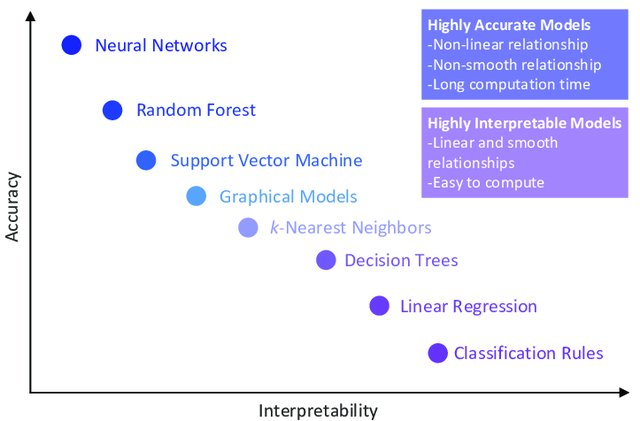
\includegraphics[scale=1.4]{images/interpretability_accuracy_tradeoff.jpg}
    \caption{The plot represented in this figure wants to highlight how different ML models are related to the trade-off between accuracy and intepretability \cite{morocho2019machine}. More a model is accurate such as Neural Network and Random Forest, more it's less interpretable due to its "black-box" nature.}
    \label{fig:trade-off}
\end{figure}
\subsection{Neural Network with Keras}
It's one of the deep learning algorithms which is based on the structure of biological neural network, where nodes represent neurons.
Nodes are connected to each others through the layers. 
In this way, every neuron of a layer is connected to neurons in the next layer.
The structure of my Neural Network is formed by 3 layers:
\begin{itemize}
    \item Input layer: Each node takes the initial data into the network and propagate information to the following layers;
    \item Output layer: It contains the result of the problem. 
    \item Hidden layer: It's actually responsible for performance and complexity of neural networks. It's placed between the output and input layers;
\end{itemize}
During the training phase, in which the network "learns", independent variables are used as input and processed through a weighted associations in which at each step produce a results which are compared to the target output. The error computed between them is successively adjusted and update following learning rules. The achievement obtained is a results increasingly similar to the values assumed by the target variable. 
For implementing it, I use Keras API from TensorFlow library.


\subsection{Machine Learning with Random Forest}
Random forests is used in regression problem, by using a structure of decision trees for making predictions. Decision trees answer to sequential questions through the routes tracked by trees.
Algorithm consists in building a certain number of random decision trees from the a bootstrap sample of the original data set (this phase is called bootstrap sampling). Then, the prediction of a certain sample is performed by following each decision trees. In a regression problem the final decision will be an averaged value from the ones obtained by each tree (phase of aggregation).
For implementing it, I use RandomForestRegressor class from sklearn library, configured with 300 random trees.
\bigbreak
In the next chapters each step will be described in depth about procedures adapted in the case of study and the results obtained.

\begin{figure}[H]
    \centering
    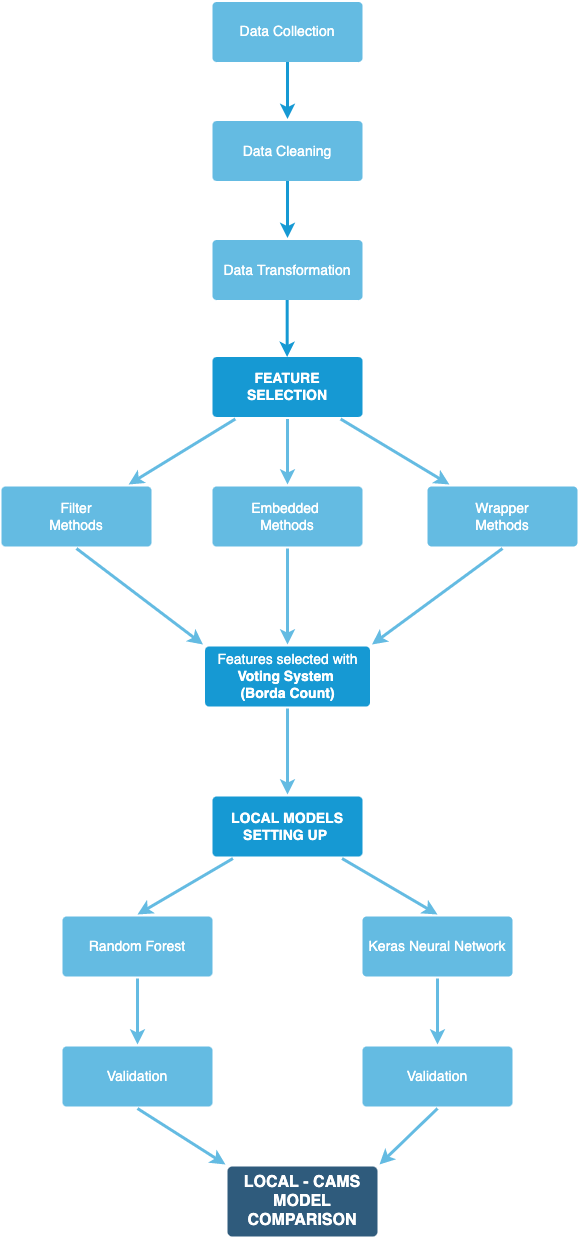
\includegraphics[scale=0.35]{images/overview.png}
    \caption{The following diagram give a general explanation of the procedure taken in this work thesis. It starts with the pre processing of the data (collection, cleaning and transformation) and continues with the selection of most meaningful variables (feature selection). \\
    After that, ML models are implemented and trained with the covariates chosen in the previous step. \\
    Finally an evaluation of the error metrics based on the validation is performed.}
    \label{fig:overview}
\end{figure}


\section{Notebook implemented}
For processing and analysing data I implemented tools collected in Python Notebooks, each one available in the D-DUST repository:
(\url{https://github.com/opengeolab/D-DUST/tree/thesis_MB}).\newline
Its essential steps are shown in figure \ref{fig:overview}.

\subsection{Computation and view of feature selection results}
In order to manage its configuration and the results obtained, a simple User Interface using ipywidgets package is built.
In this interface there are 2 sections:
\begin{itemize}
\item Feature Selection scores: they are graphically shown using multiple barplot, one for each data set previously selected. Barplot are implemented with the use of Plotly library; 
\item Options: in this box is possible to configure the feature selection input:
\begin{itemize}
\item target variable. Variable usable are the ones coming from ARPA ground sensors;
\item value of the Variance Threshold for discarding meaningless variable before FS (optional);
\end{itemize}
and the output:
\begin{itemize}
\item choice of method for visualize its own scores;
\item results normalization (optional);
\item order of the scores by descending order or by labels;
\item scale of Y-axis (regular or logarithmic);
\end{itemize}
\end{itemize}
A pseudo code of how the notebook works is atteched.
\begin{verbatim}
for each configuration in configurations
    for each period in periods
        #Data acquisition
        grid = input(period)
        grid = buffer_knn(grid)
        data_cleaning(grid)
        grid = VarianceThreshold(grid, 0.1)
        X, Y = get_variables(grid, target_variable)
        #Feature selection phase
        results = compute_feature_selection(X, Y)
    results = borda_count_algorithm(results)
    #results are stored externally in .csv files
    export_tocsv(results) 
    #results exported will have the feature ordered with respect
    #the score obtained with Borda Count algorithm
\end{verbatim}
\begin{figure}[H]
    \centering
    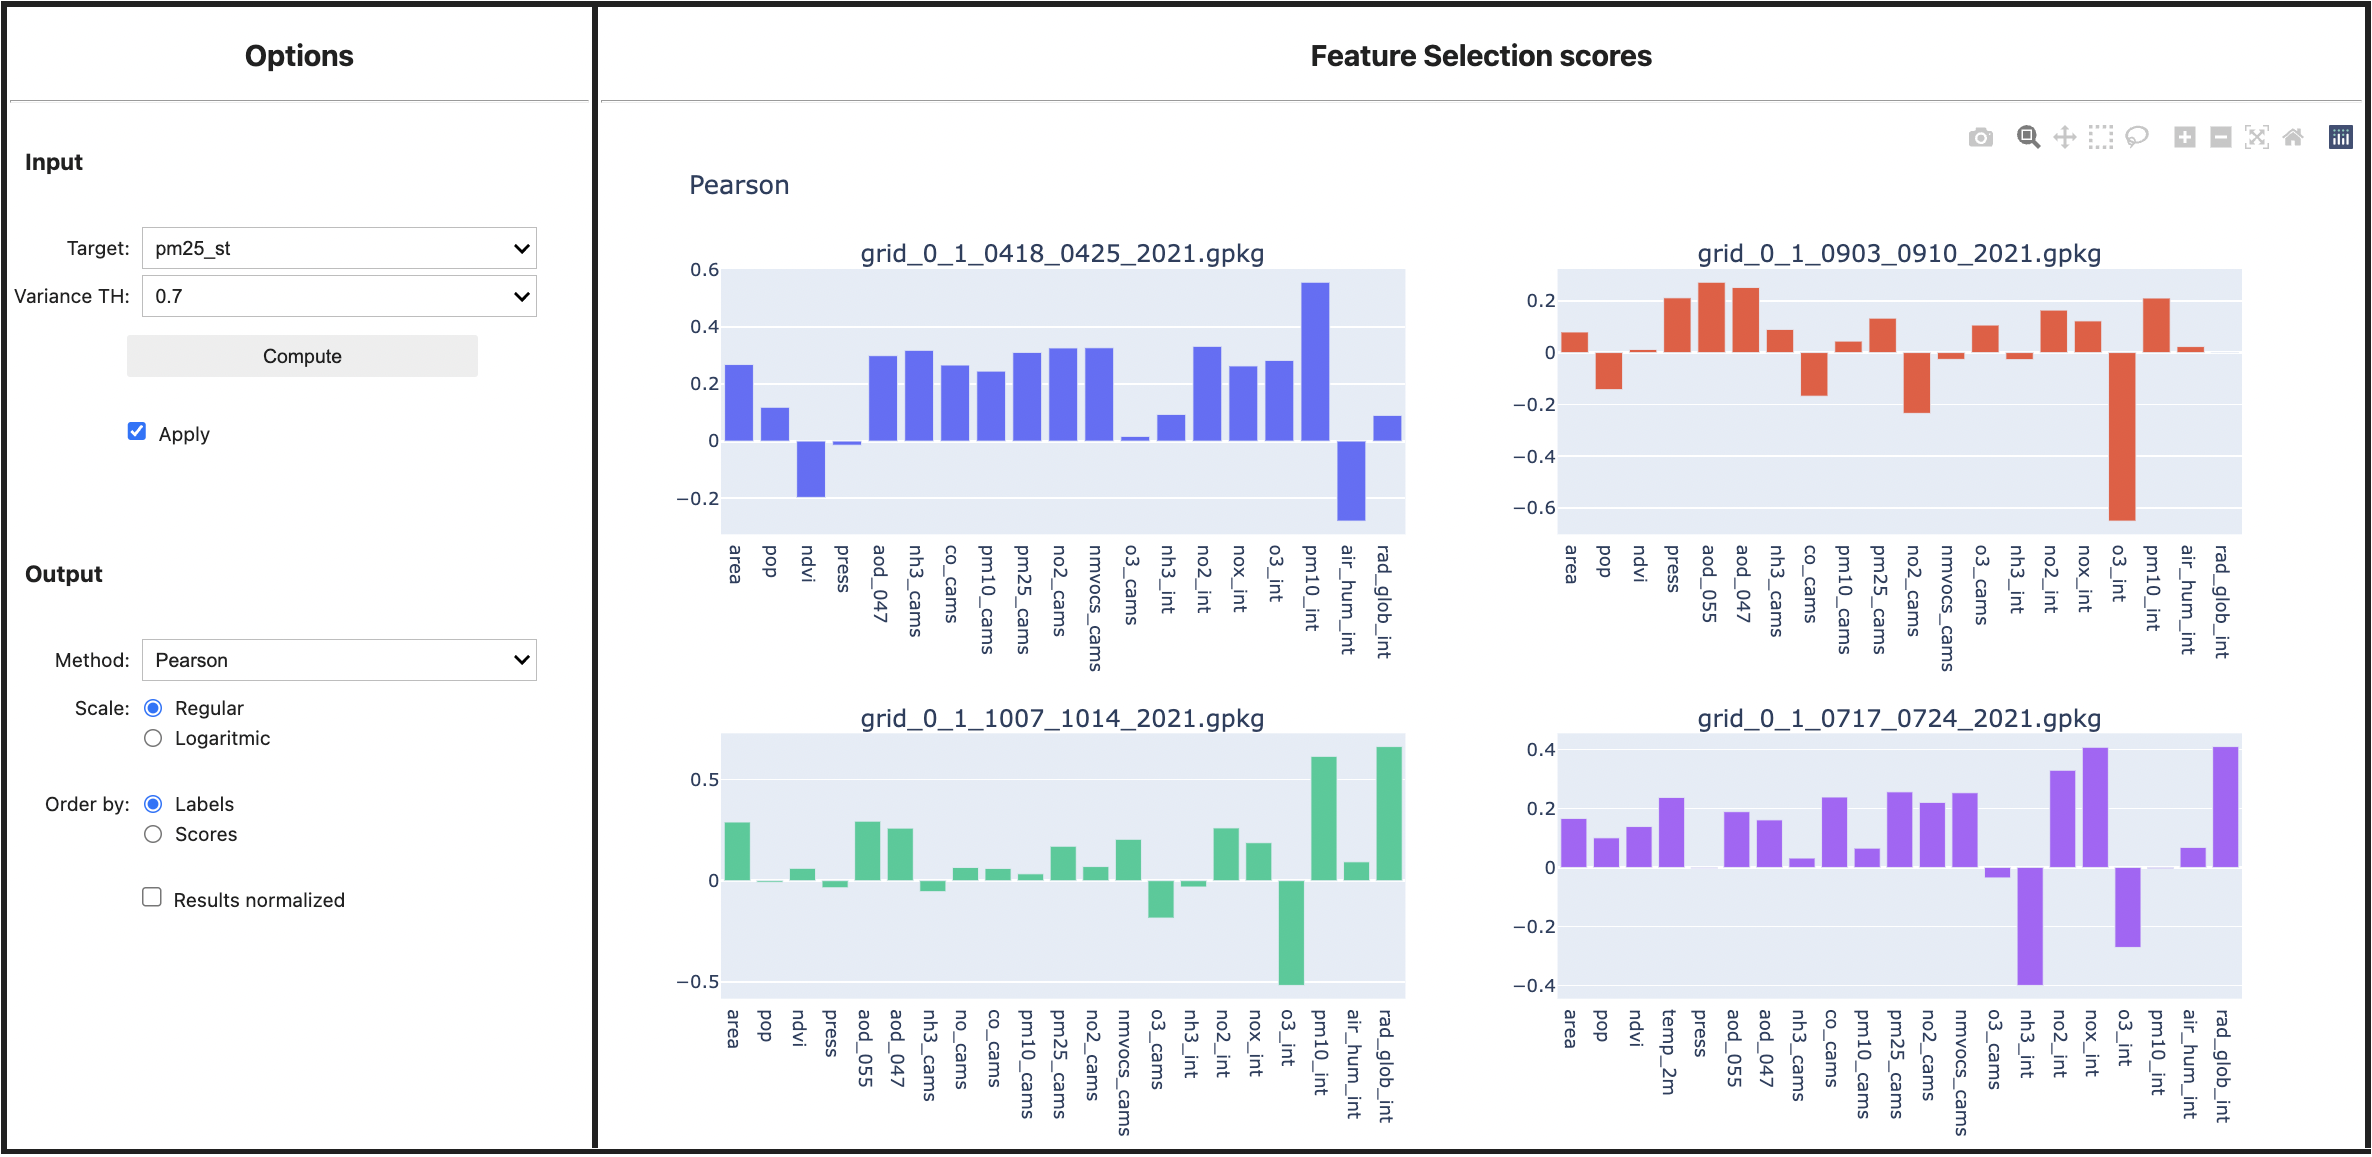
\includegraphics[scale=0.40]{images/notebook.png}
    \caption{Overview of the notebook implemented for FS procedure.}
    \label{fig:notebook}
\end{figure}

In the notebook are present also cells which aims to export FS results.

\subsection{Computation and view of ML models results}
For build I use 2 different notebook for the evaluation of the Neural Network (\href{https://github.com/opengeolab/D-DUST/blob/thesis_MB/notebooks/Keras_prediction_model.ipynb}{link}) and the Random Forest model (\href{https://github.com/opengeolab/D-DUST/blob/thesis_MB/notebooks/RandomForest_prediction_model.ipynb}{link}). 
It possible to set these parameter before running the model:
\begin{itemize}
    \item NUMBER\_OF\_COVARIATES: It's number of the n features with the highest Borda Count score take as input for the model;
    \item TARGET: It represents the target variable to be predicted by the model;
\end{itemize}
\begin{verbatim}
for each configuration in configurations
    results = []
    for each period in periods
        #Data acquisition
        grid = input(period)
        grid = buffer_knn(grid)
        data_cleaning(grid)
        X, Y = get_variables(grid, TARGET)
        X = get_n_columns(NUMBER_OF_COVARIATES)
        #Modelling in which training and validation is performed using k-fold
        model = new()
        model.training(X, Y)
        res = model.validation(X, Y)
        results.append(res)
    
    #results are stored externally in .csv files
    export(avg(results1))
    export(avg(results2))
 
\end{verbatim}

Each one of them imports the feature selected from the previous notebook and export the accuracy evaluation of the k-fold cross validation externally. \par
The results are subsequently opened and shown with \href{https://github.com/opengeolab/D-DUST/blob/thesis_MB/notebooks/model.ipynb}{this other notebook} through the use of widgets (\ref{fig:view}.
\begin{figure}[H] 
    \centering
    \subfloat[Drop-down widgets.]{%
        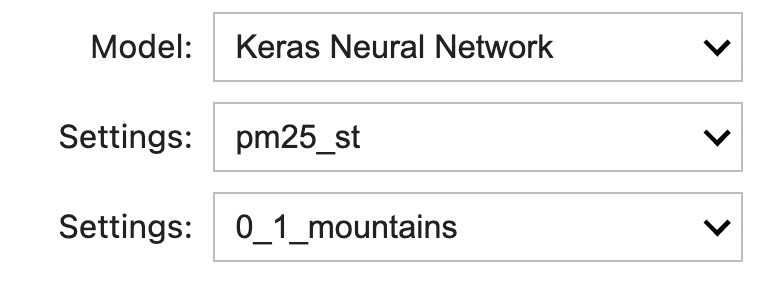
\includegraphics[width=0.5\textwidth]{images/dropdown.png}%
        %
        }%
    \hfill%
    \subfloat[Table with the results selected.]{%
        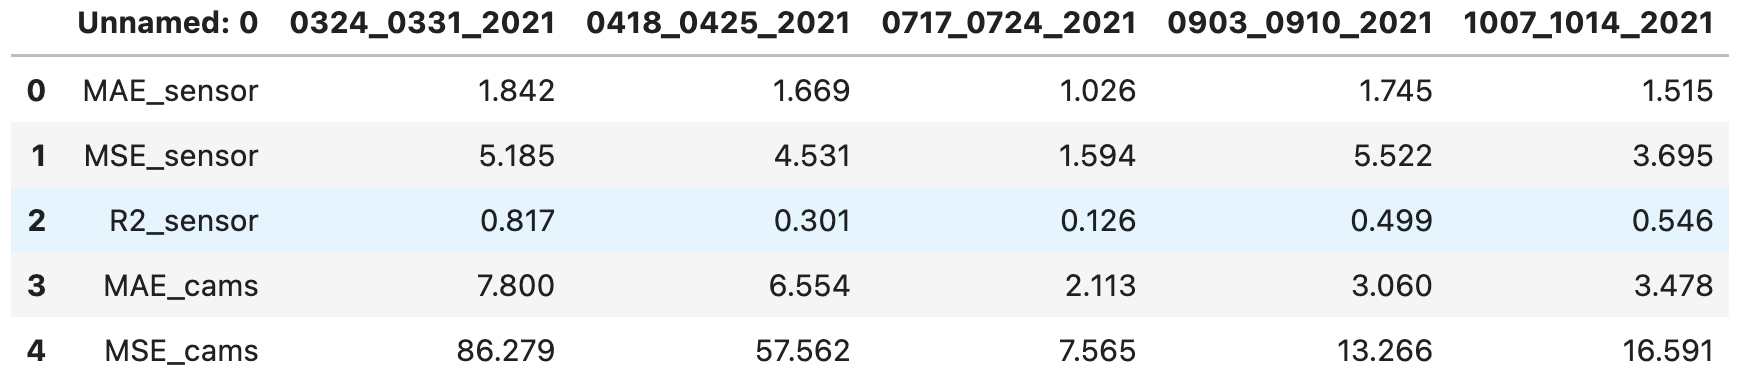
\includegraphics[width=0.5\textwidth]{src/images/table.png}%
        %
        }%
    \caption{In these images is illustrated how the notebook view for viewing the validation results works. It sufficient to select the target variable, resolution and configuration desired and with the an interactive option provided by ipywidgets library the results are provided through a table.}
    \label{fig:view}
\end{figure}

An overview of the order in which the different notebooks are used in my work thesis is illustrated in the figure .
\begin{figure}[H]
    \centering
    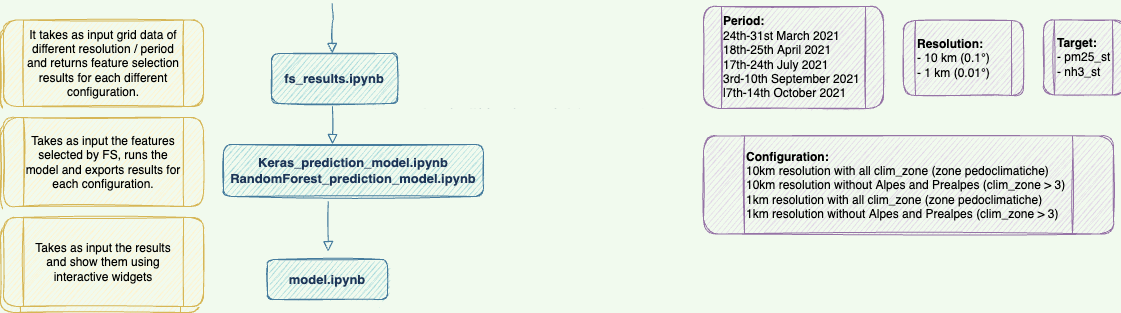
\includegraphics[scale=0.35]{images/overview _notebooks.png}
    \caption{The following diagram give a general explanation of the sequence of the notebooks which are used. It starts with fs\_results.ipynb which aims to collect, clean, transform and select the most meaningful variables through the Feature Selection). \\
    After that, Keras\_prediction\_model.ipynb and RandomForest\_prediction\_model.ipynb are used to implement ML models which are trained with the covariates chosen in the previous step. \\
    Finally the results of the error metrics based on the validation are provided by model.ipynb. 
    The results collected are each one configured with an initial VariancaThreshold method with 0.1 value}
    \label{fig:notebooks}
\end{figure}